\documentclass[12pt,fleqn,a4paper,oneside]{mybook} %Final!!!
%\documentclass[11pt,fleqn,a4paper,draft]{mybook} %DRAFT - highlights overflow, leaves out images

%\usepackage{microtype}
\usepackage[slovak]{babel}
\usepackage[utf8]{inputenc}
\usepackage[T1]{fontenc}
\usepackage[normalem]{ulem}
\usepackage{mathtools}  					
\usepackage{graphicx}
\usepackage{subfigure}
\usepackage{enumerate}
\usepackage{etoolbox}                       %Problematic URL in reference
\apptocmd{\sloppy}{\hbadness 10000\relax}{}{}%Removes badness warnings
%This is to remove warnings resulting by otherwise OK URL's
\usepackage[hyphens]{url}
\usepackage{notes}
\usepackage{indentfirst}






%This custom command defines how the literal menus look like.
\newcommand{\gui}[1]{{\emph{#1}}} %Gui commands, icon names, buttons
 % All code, functions, variables are typed like this
\newcommand{\code}[1]{{\lstinline[columns=fixed]{#1}}}

\newcommand{\angl}[1]{{\footnote{\emph{angl.}\ {#1}}}} %Shorthand english equivalent


\usepackage[left=25mm,right=25mm,top=25mm,bottom=25mm,paperwidth=210mm,paperheight=297mm,includehead]{geometry}

\usepackage{titlesec}
\titleformat{\chapter}[hang]{\normalfont\huge\bfseries}{\thechapter}{1em}{}


\DeclarePairedDelimiter{\diagpars}{(}{)}
\newcommand{\diag}{\operatorname{diag}\diagpars}

\let\oldhat\hat
\renewcommand{\vec}[1]{\boldsymbol{\mathbf{#1}}}
%\renewcommand{\hat}[1]{\oldhat{\boldsymbol{\mathbf{#1}}}}


\usepackage{amsthm}
\usepackage{etoolbox}% http://ctan.org/pkg/etoolbo
\theoremstyle{definition}
\newtheorem{exmp}{Pr\'{i}klad}[chapter]
\AtEndEnvironment{exmp}{\null\hfill\qedsymbol}

\usepackage{listings,color} 			    %To list Matlab code
\definecolor{mygrey}{gray}{0.5}	        %Define a gray color
\lstset{
basicstyle=\ttfamily,
numbers=none,
commentstyle=\color{mygrey},
breaklines=true,
}
%extended Matlab language
\lstdefinelanguage{exMatlab}[]{Matlab}      %Defining expanded Matlab
{morekeywords={rng,pyulear,plot,hold,randn,filter,length,abs,periodogram,fft,sin,randn,xcorr,fminsearch,dlqr,predmodelqp,dlyap,ones,linprog,quadprog,optimset,qpOASES,qpOASES_sequence,sysStruct,probStruct,mpt_control,volume,hull,extreme,mpt_exportc,mpt_getInput,sdpvar,blkdiag,sdpsettings,solvesdp,geomean,double},
sensitive=true,
alsoletter={_}
}



\pagestyle{empty}

\begin{document}
%%%%%%% Zaciaatok %%%%%%%%
\renewcommand\thepage{\roman{page}}
\pagenumbering{roman}
\thispagestyle{empty}

\noindent \begin{center}
\textbf{{\large{}SLOVENSKÁ TECHNICKÁ UNIVERZITA V BRATISLAVE}}\\
\textbf{{\large{}STROJNÍCKA FAKULTA}}\textbf{\large{} }\\
\vspace{3cm}
\par\end{center}

\noindent \begin{center}
\vspace{3cm}
\par\end{center}



\begin{center}
\textbf{\textsc{\Large{}MIKROPROCESOROVÁ TECHNIKA}}\\
\par\end{center}{\Large \par}

\begin{center}
\textbf{\large{}ZÁVEREČNÁ PRÁCA: OVLÁDAČ HLASITOSTI  }\\
\par\end{center}{\large \par}





\vfill
\noindent \textbf{\normalsize{}2022} 
\noindent \textbf{\normalsize{}  Samuel Suchý}
\noindent \textbf{\normalsize{}  Martin Košťál}
\noindent \textbf{\normalsize{}  Lukáš Šipoš}
\noindent \textbf{\normalsize{}  Michal Bíro}
\noindent \textbf{\normalsize{} Peter Tibenský}
\cleardoublepage

\listoffigures
%%%%%% \chapter*{Predhovor}
\thispagestyle{empty}

Myslel som si že ma táto téma bude baviť. Až pokial som si neuvedomil, že to nebude až také jednoduché... 

Už od malička ma fascinovala elektronika a všetko čo sa vedelo pohybovať a ja som to vedel riadiť. Volba tejto bakalárskej práce preto bola jasnou voľbou. 

\cleardoublepage

 %%%%%%
\tableofcontents
\thispagestyle{empty}
\cleardoublepage

%%%%%% Jednotlive kapitoly %%%%%%%%%
\pagestyle{plain}
\pagenumbering{arabic}
\setcounter{page}{1}


\chapter*{Úvod}
\label{UVOD}
\addcontentsline{toc}{chapter}{Úvod}

Problém veľa moderných filmov je, že hladiny zvuku nie sú konzistentné počas celého trvania filmu, najbežnejší prípad je omnoho hlasnejšia hudba ako zvuk konverzácií, čo núti ustavične upravovať zvuk pomocou ovládača. Tento problém nastáva, pretože zvuk moderných filmov je prispôsobený pozeraniu v kinách a nie na domáce pozeranie.

Jedno z riešení je zapnutie dynamickej kompresie zvuku v televíznom prijímači, avšak nie každý televízor má túto funkciu. Naše zariadenie ponúka riešenie pre televízory bez tejto funkcie.

Princíp fungovania nášho zariadenia je založený na prijímaní signálu z mikrofónu, ktorého výška určuje či budeme zvyšovať alebo znižovať hlasitosť televízora a tým meniť výstup infračervenej LED mierenej na televízor




\chapter{Hardware}
\section{Schéma zapojenia}
Schéma zapojenia je pomerne jednoduchá obr.\ref{OBRAZOK 1.1}. Jej najdôležitejšiu časť tvorí operačný zosilňovač MCP602 obr.\ref{OBRAZOK 1.2}. Operačný zosilňovač je jednosmerne viazaný elektronický zosilňovač napätia s vysokým ziskom s diferenciálnym vstupom a zvyčajne s jednosmerným výstupom. V tejto konfigurácii optický zosilňovač vytvára výstupný potenciál (vzhľadom na zem obvodu), ktorý je zvyčajne 100 000-krát väčší ako rozdiel potenciálov medzi jeho vstupnými svorkami.

\begin{figure}[!tbh]
\centering

\includegraphics[width=\textwidth]{obr/schema.png}
\caption{schéma zapojenia.}\label{OBRAZOK 1.1}
\end{figure}

Na tento zosilňovač máme pripojený elektrický kondenzátorový mikrofón obr.\ref{OBRAZOK 1.3}. Skladá sa z dvoch platní, jednej pevnej a druhej pohyblivej. Vibrácie vzduchu sa transformujú na posun pohyblivej membrány, ktorá vytvára zmenu elektrického potenciálu. Túto zmenu zachytáva  snímač, ktorý následne vysiela elektrický signál. Elektrický signál sa zosilní a následne je spracovaný v arduine.

\begin{figure}[!tbh]
\centering
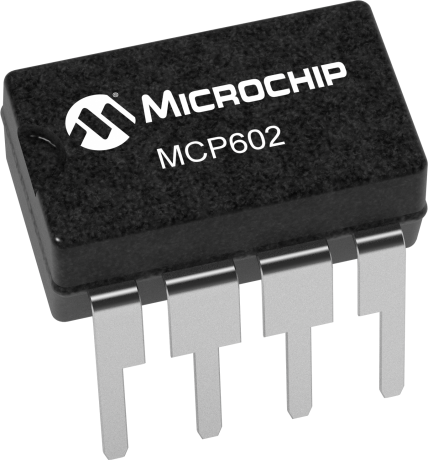
\includegraphics[width=8cm]{obr/mcp.png}
\caption{{operačný zosilňovač MCP602.\cite{mcp}}}\label{OBRAZOK 1.2}
\end{figure}

\begin{figure}[!tbh]
\centering
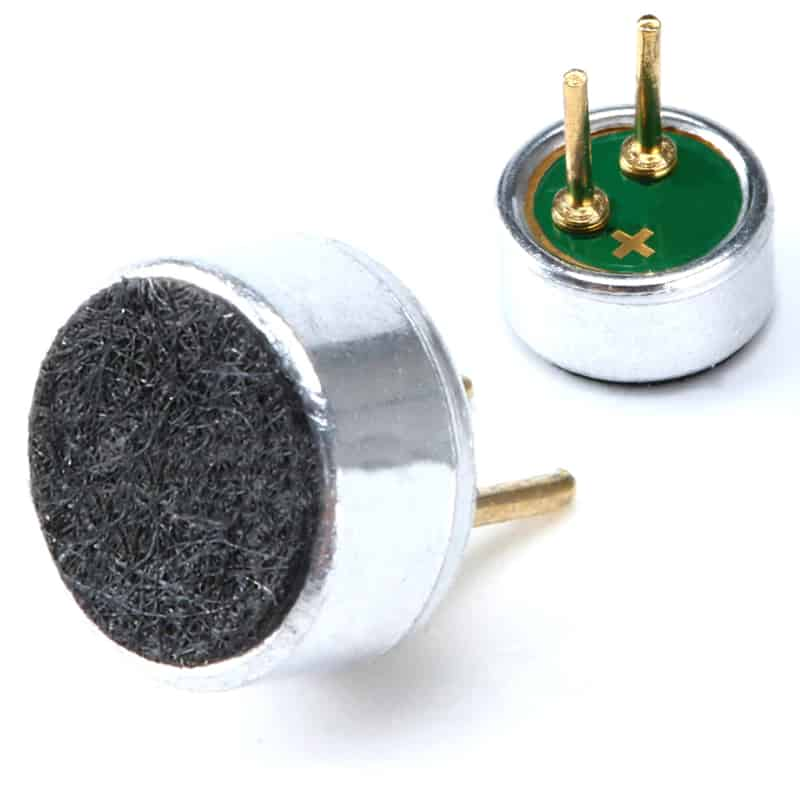
\includegraphics[width=7cm]{obr/mike.jpg}
\caption{{elektrický kondenzátorový mikrofón.\cite{mike}}}\label{OBRAZOK 1.3}
\end{figure}

Ďalšou kritickou časťou systému je infračervená LED dióda, pomocou ktorej posielame signály potrebné na ovládanie televízora. Je dôležité podotknúť že nie všetky televízory resp. ovládače, fungujú na princípe infračervenej LED diódy, avšak v dnešnej dobe pracuje na tomto princípe väčšina zariadení. LED dióda vysiela špeciálne príkazy pomocou modulácie dĺžok medzier medzi vyslanými signálmi ktoré následne zachytáva a spracováva televízor.

Následne sa na doske nachádzajú aj 2 potenciometre ktoré slúžia na nastavovanie hodnôt potrebných pre správne fungovanie API a 2 LED diódy, jedna zelená, druhá červená, ktoré slúžia len na vizuálnu kontrolu fungovania systému keďže infračervené lúče vysielané IR LED diódou sú pre naše oči neviditeľné.

Na schéme môžeme takisto vidieť IR snímač VS1838B ktorý sme chceli využiť na zapisovanie signálov na zvyšovanie a znižovanie hlasitosti. Na spustenie tejto funkcie slúži tlačidlo s názvom BUTTON ktoré je tiež viditeľné na schéme. Žiaľ, túto funkciu sa nám nepodarilo úspešne implementovať do nášho kódu. Problémom pri spolupráci na projekte bol lockdown a nemožnosť spoločnej práce v reálnom svete ale iba pomocou online komunikácie. Práca s hardwarom tak bola náročnejšia a testovanie kódu, ktorý sme napísali, bolo obmedzené.

Hlavným nedostatkom tohto kódu bolo správne zapísanie získaných hodnôt do funkcie IRsenderu. Kód sme úspešne detegovali a vedeli ho uložiť do pamäte EEPROM, no následné zapísanie uloženého kódu a jeho poslanie nefungovalo ani po mnohých iteráciách. Kód bol teda na \verb|99%| funkčný, ale jeho najdôležitejšia časť, posielanie signálov, nám nechcela fungovať. V situácii kedy by bolo na projekt viacej času, túto funkciu by sme radi implementovali do ovládača hlasitosti.






\section{Prototyp zapojenia pomocou breadboardu}

Na otestovanie správnosti a funkčnosti kódu bol zostavený model systému na breadboarde obr.\ref{OBRAZOK 1.4}. Systém po niekoľkých iteráciách softwaru a hardwaru fungoval s vysokou presnosťou a bolo možné ho vyladiť podľa potrieb užívateľa. Na ovládanie prvej verzie ovládača hlasitosti sme použili Arduino UNO ktorého sériový port a vykresľovanie meraných veličín nám veľmi uľahčili proces vylepšovania kódu.

\begin{figure}[!tbh]
\centering
\fbox{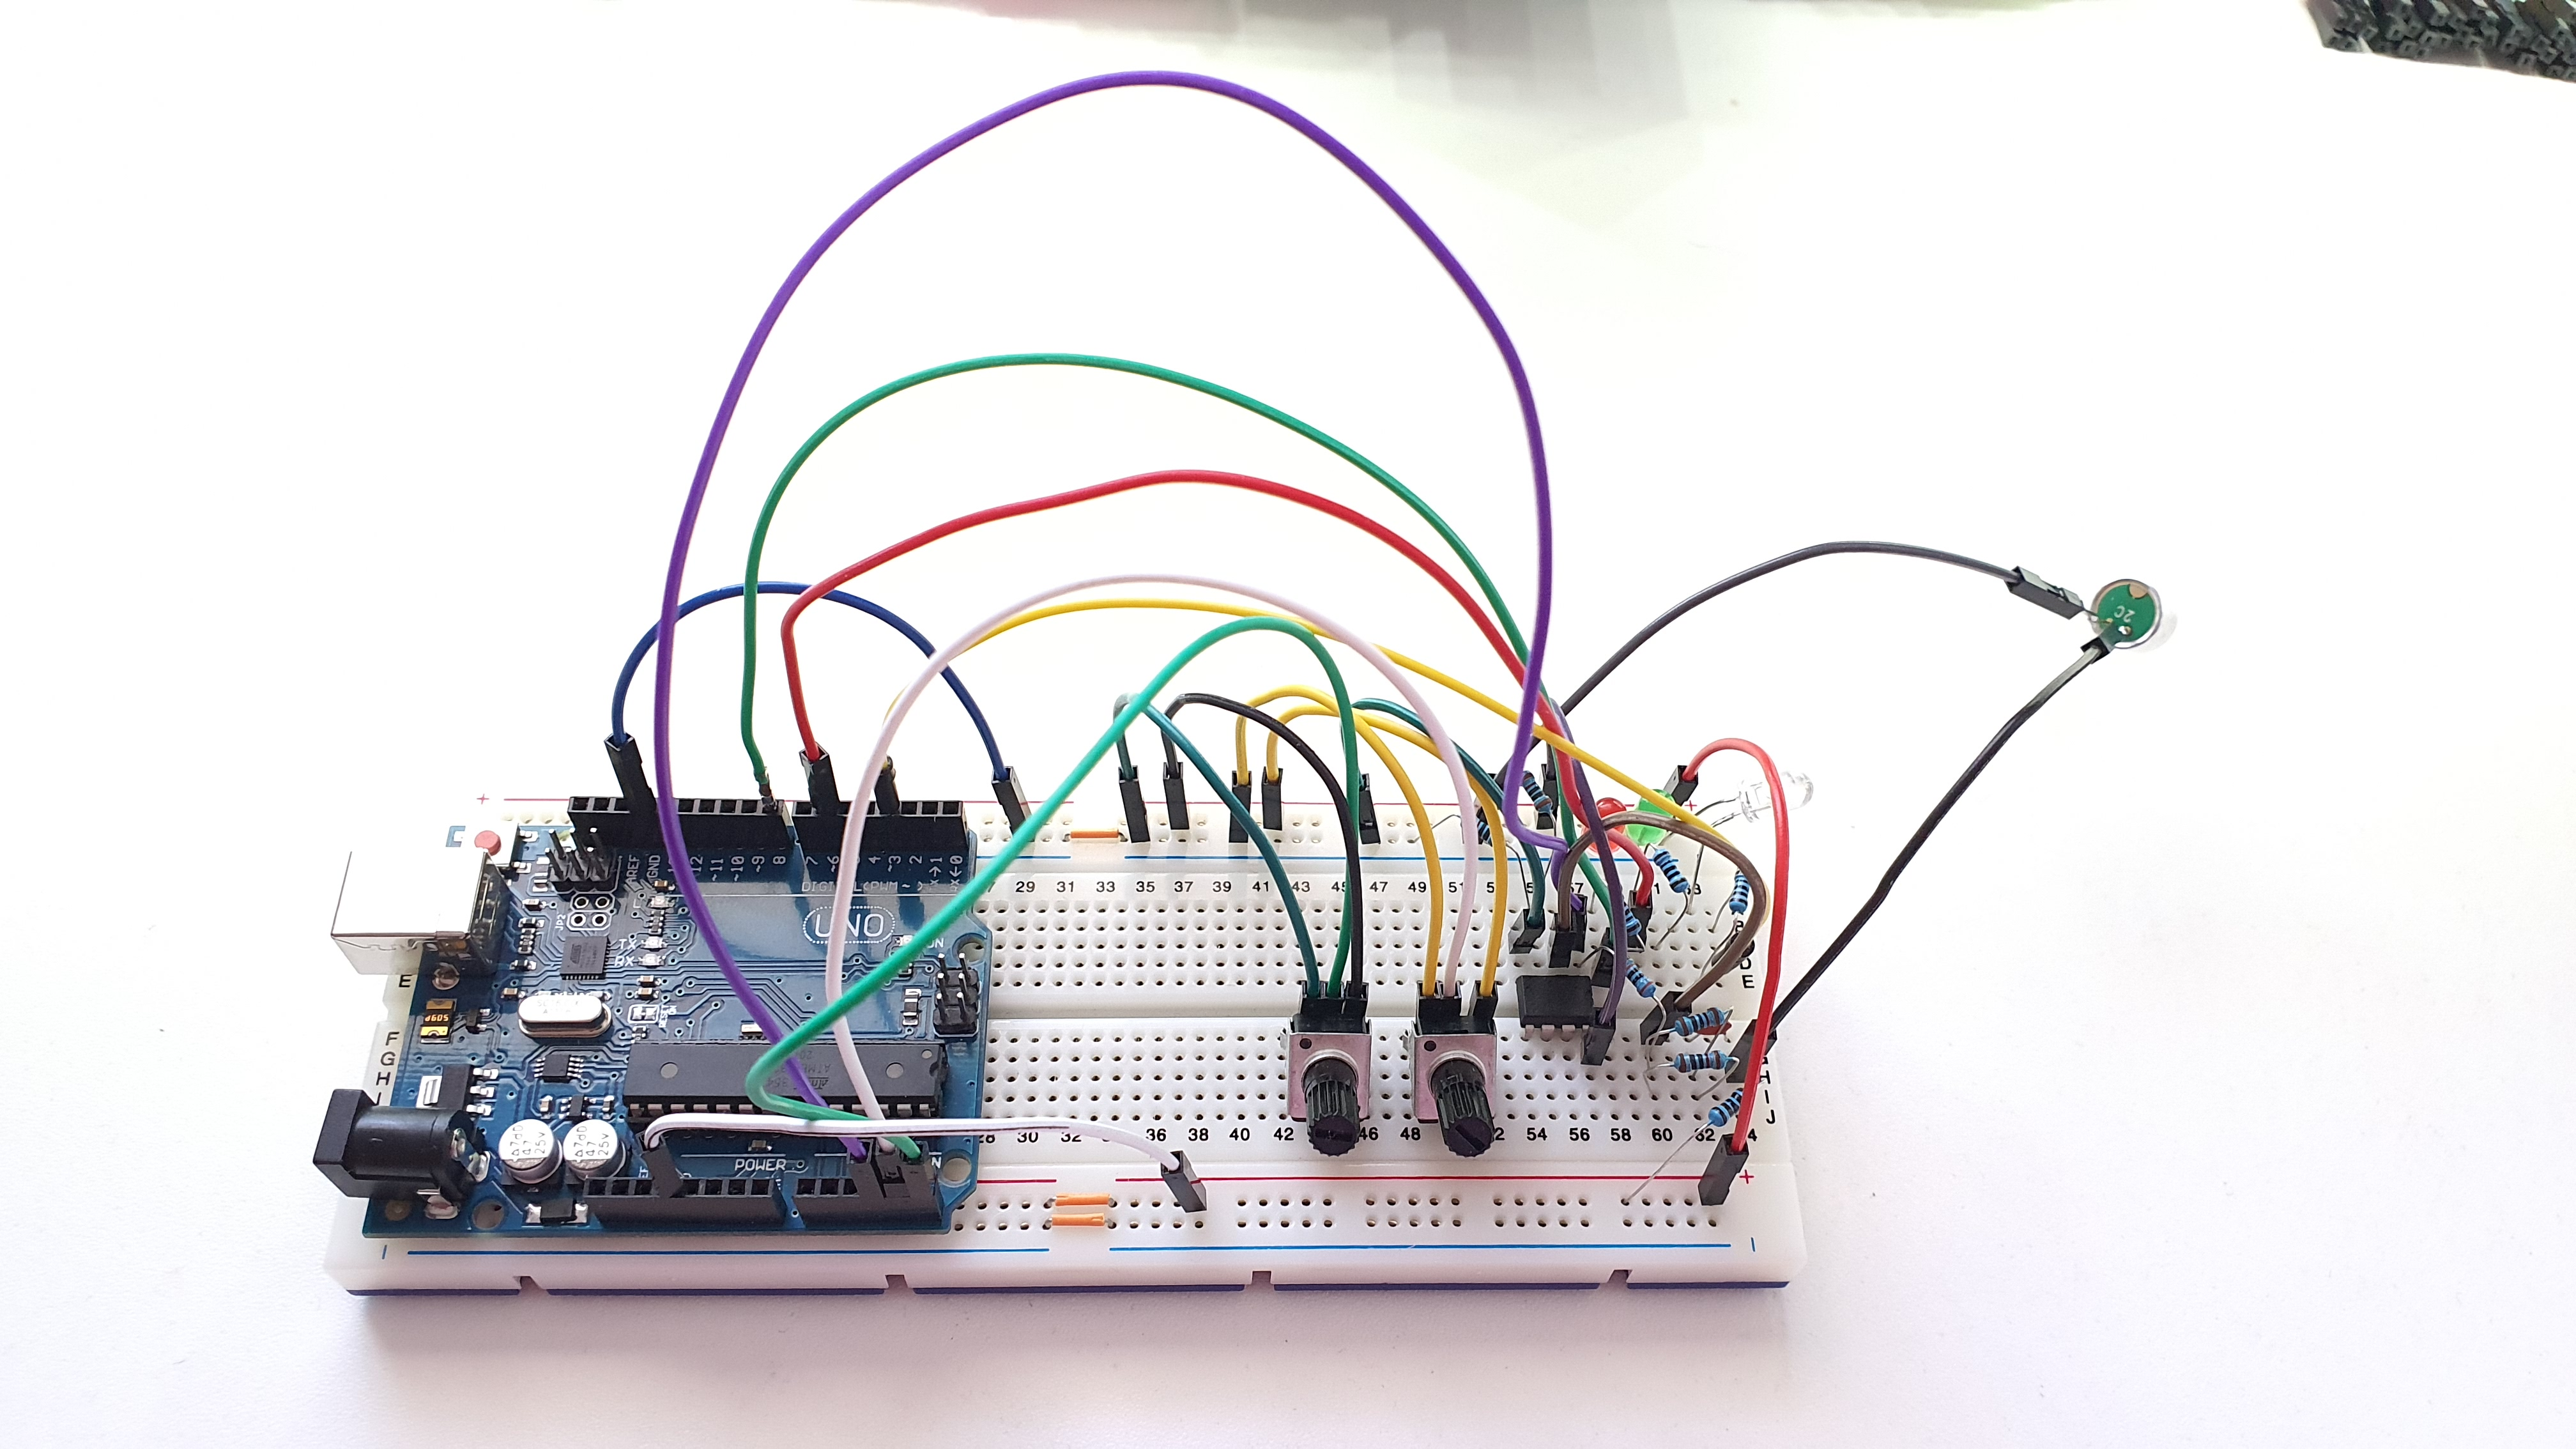
\includegraphics[width=12cm]{obr/breaduno2.jpg}}
\caption{Zapojenie na breadboarde.}\label{OBRAZOK 1.4}
\end{figure}

\begin{figure}[!tbh]
\centering
\fbox{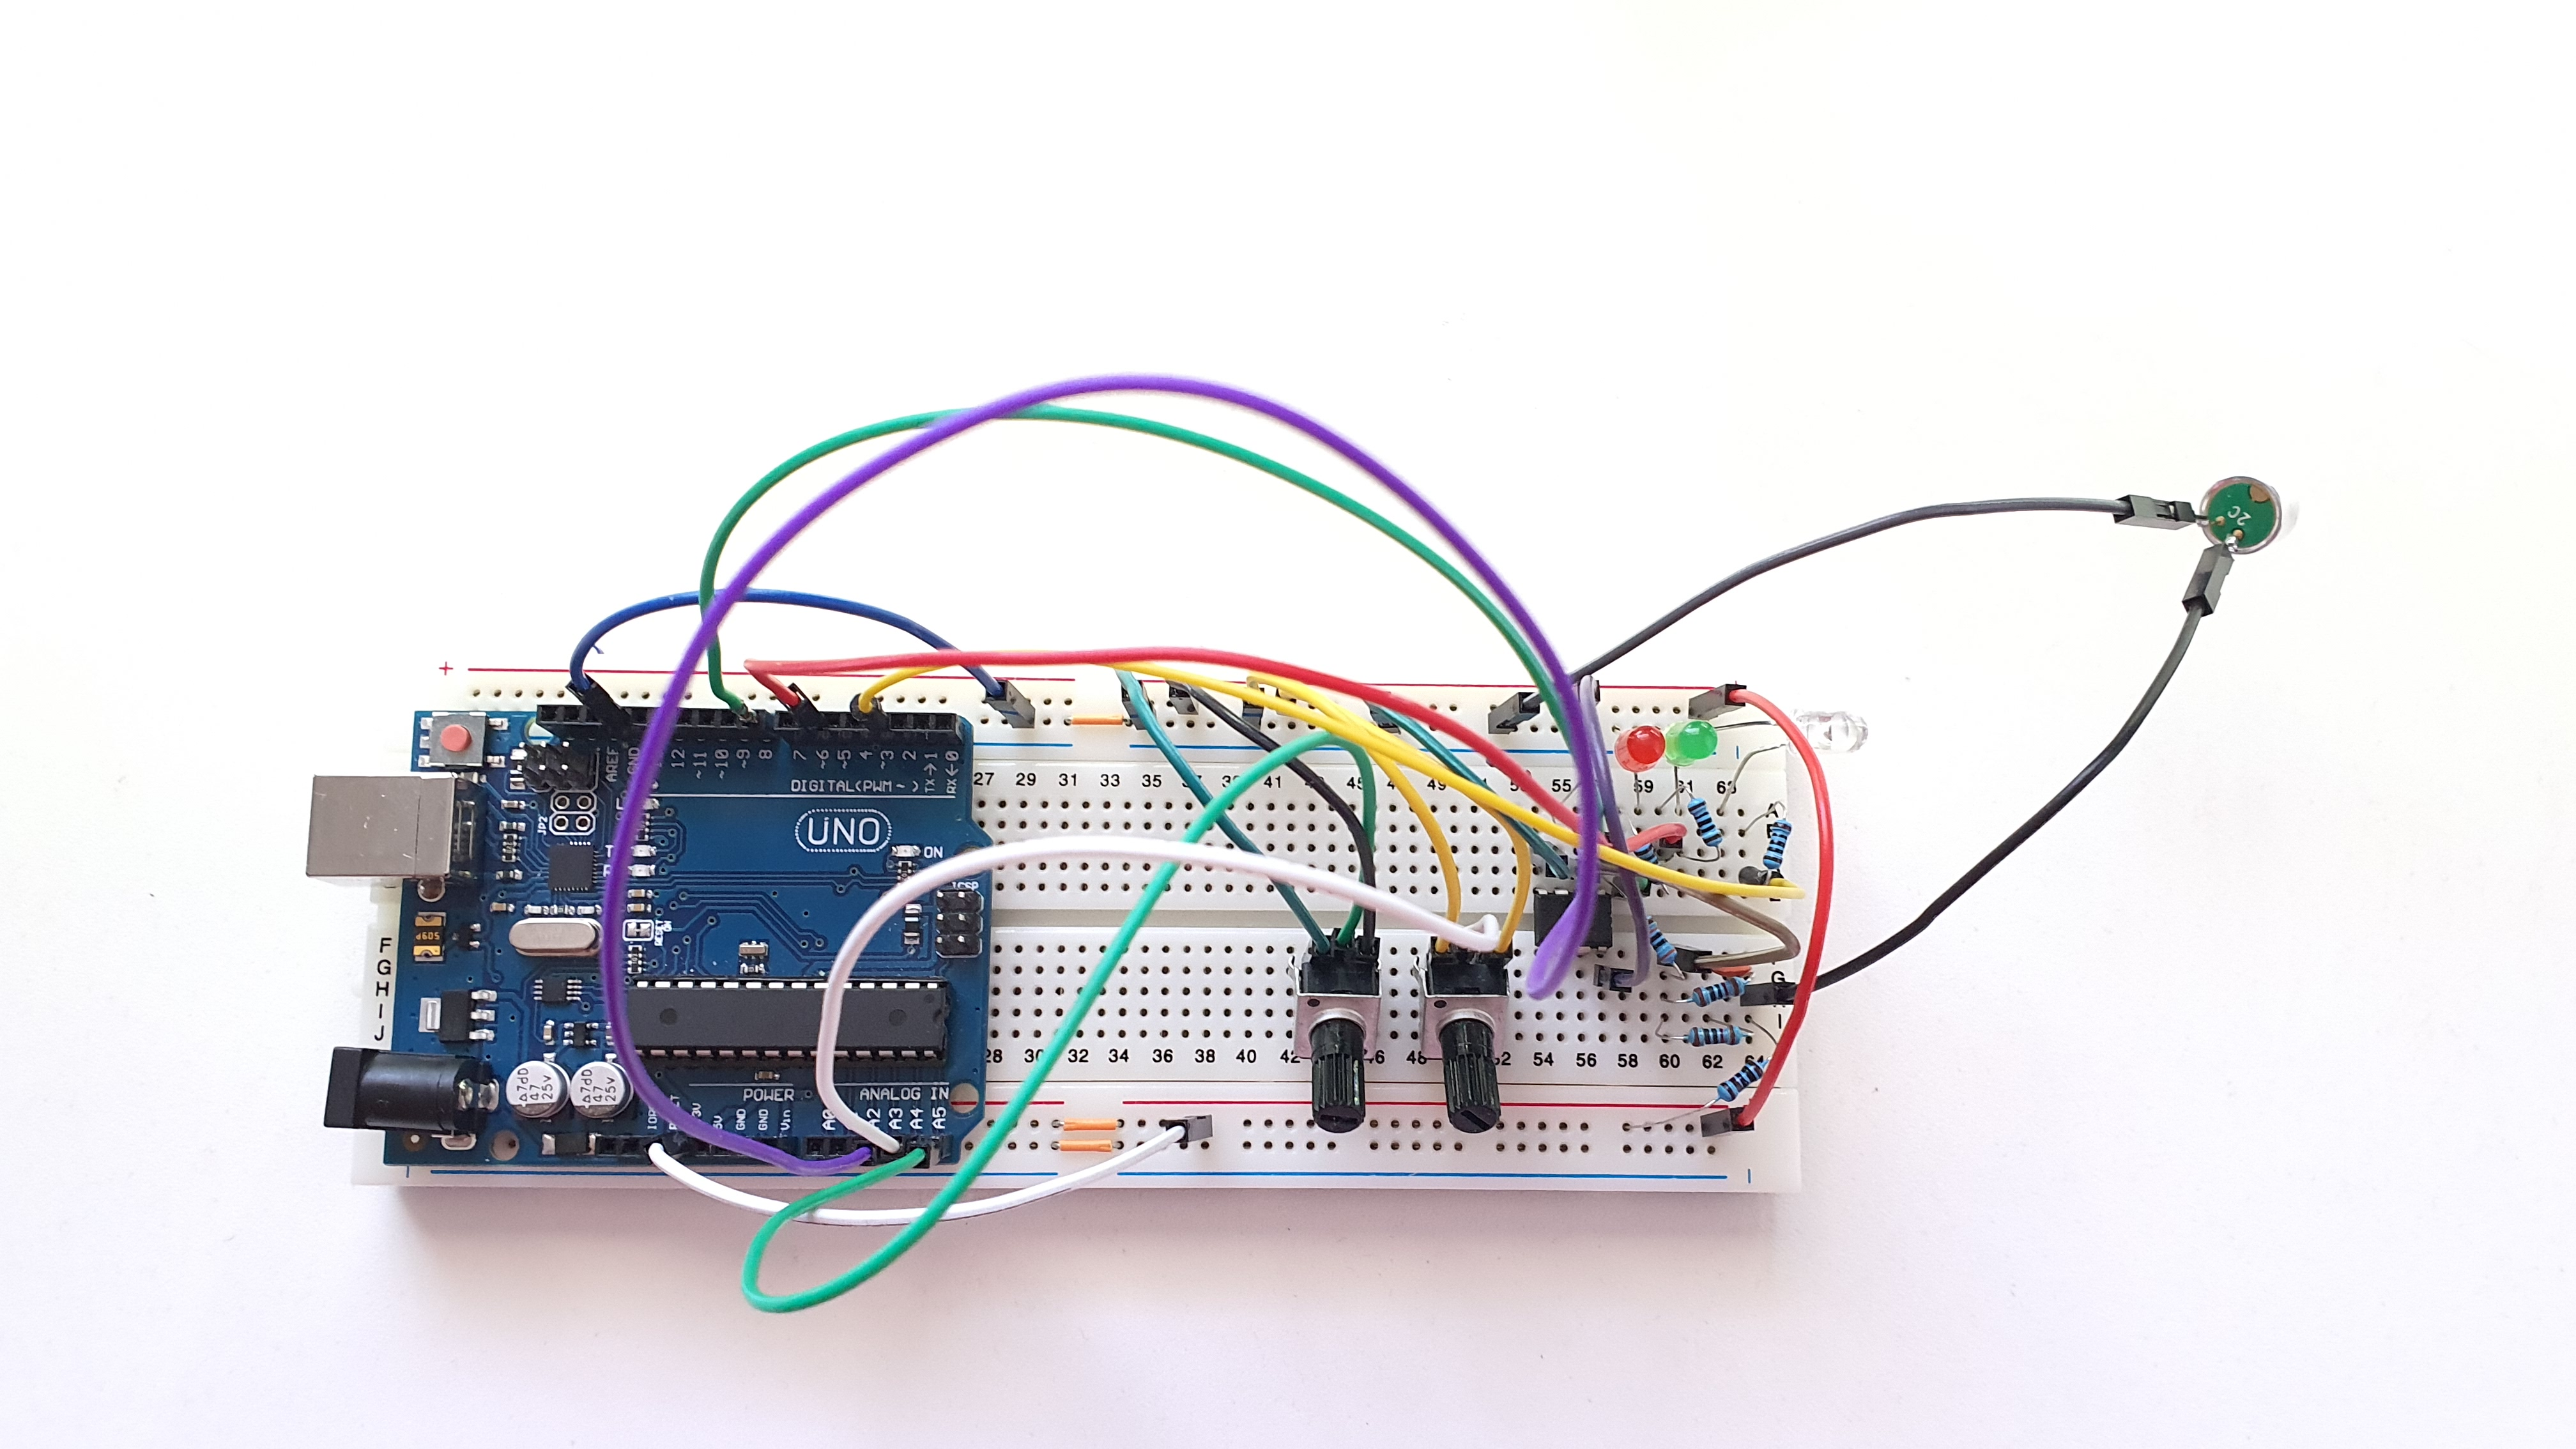
\includegraphics[width=12cm]{obr/breadunohorepohlad.jpg}}
\caption{Zapojenie na breadboarde.}\label{OBRAZOK 1.4}
\end{figure}



\section{Prototyp zapojenia pomocou jednostrannej prototypovej dosky}

Ako ovládací prvok v 2. generácii obr.\ref{OBRAZOK 1.5} systému sme si zvolili Arduino pro mini, ktorého rozmery a cena boli vyhovujúce pre naše potreby. Schéma zapojenia pre Arduino pro mini je totožná so zapojením pre Arduino UNO až na to, že Arduino pro mini sme sa rozhodli napájať pomocou 3,7V lítiovej batérie zapojenej v kontrolóri nabíjania batérie 03962A. Na správne fungovanie lítiovej batérie je kritické nedovoliť batérii úplne sa vybiť. Z tohto dôvodu budeme pomocou analógového pinu A2, merať napätie batérie a pri kritickom napätí sa spustí blikanie led diódy obr.\ref{OBRAZOK 1.7}, ktorá indikuje nutnosť nabitia batérie pomocou mikro USB portu obr.\ref{OBRAZOK 1.6}.

\begin{figure}[!tbh]
\centering
\fbox{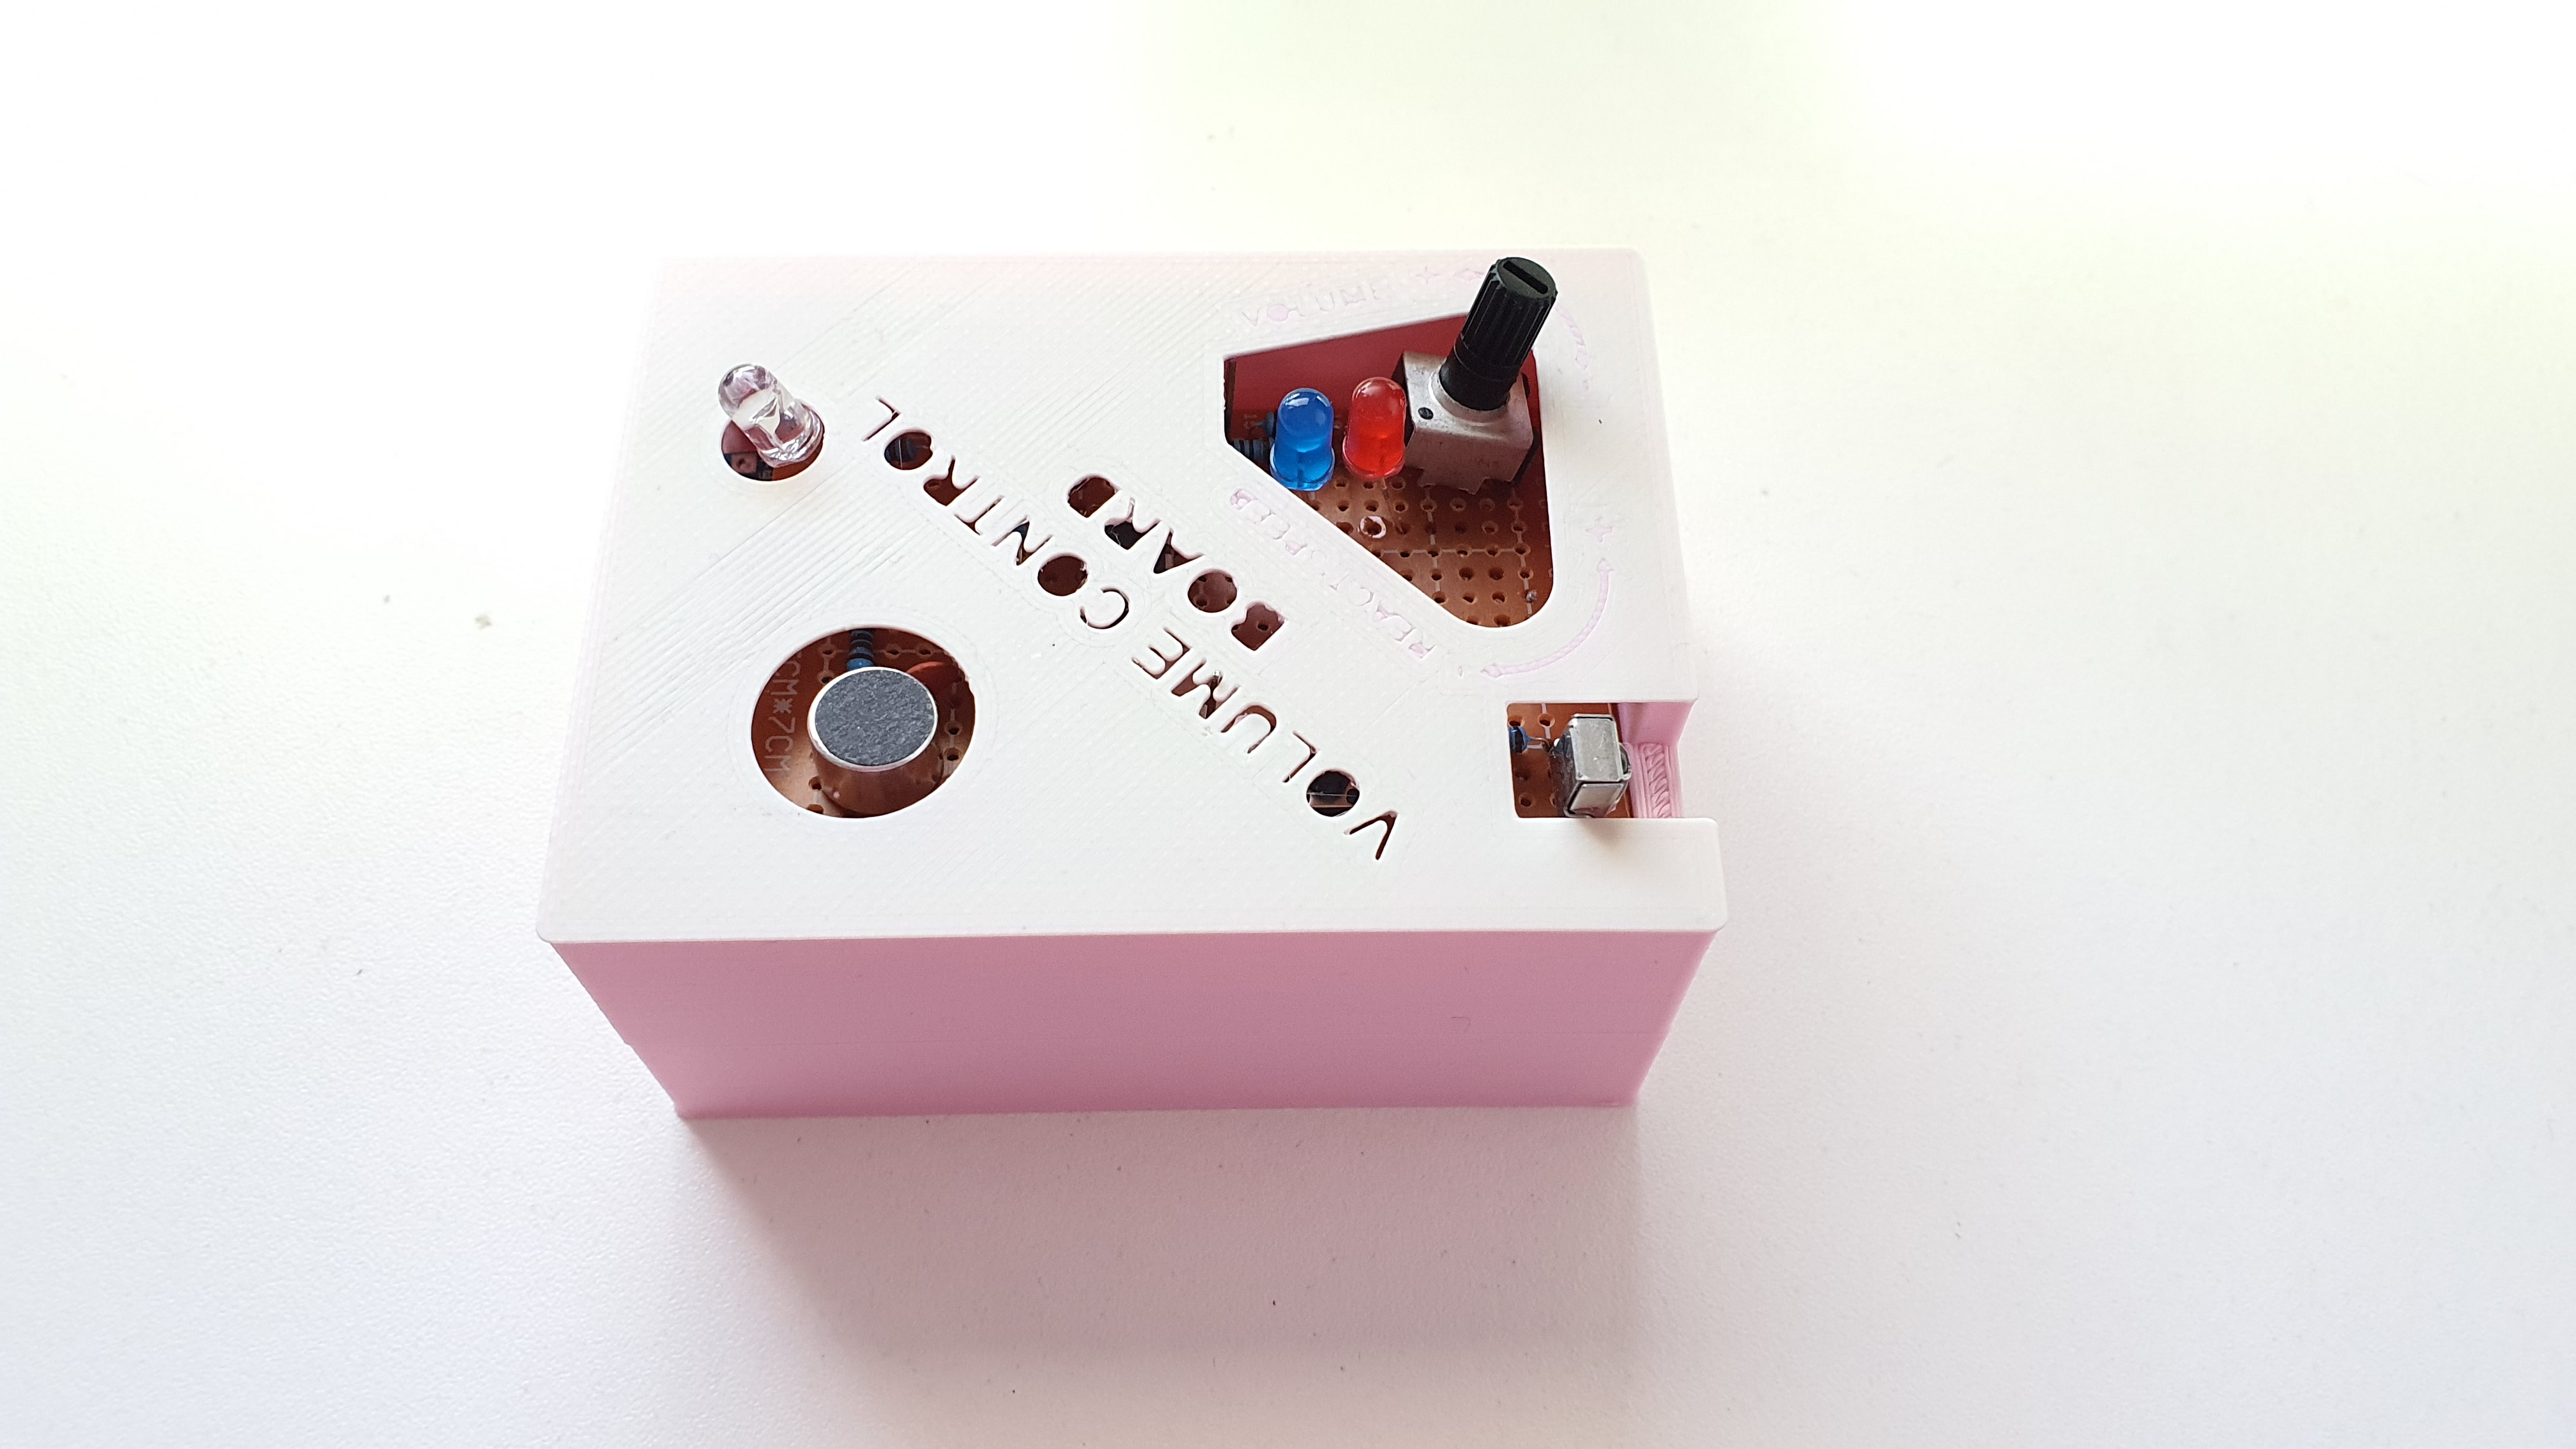
\includegraphics[width=\textwidth]{obr/obaltopuhol.jpg}}
\caption{model ovládača aj s obalom.}\label{OBRAZOK 1.5}
\end{figure}

Prototyp číslo 2 fungoval počas testovania správne a všetky funkcie sme vyladili priamo pre tento systém. Avšak pred odovzdaním projektu sa vyskytol problém so zapojením obvodov a výstupy do Arduina prichádzali v zlom tvare obr.\ref{OBRAZOK 1.8}. Problém sme odhadli na skrat medzi súčiastkami zapojenia kedy sa do výstupu mikrofónu pridával neznámy šum, ktorý znehodnotil výsledky merania mikrofónu. Chybu sme sa snažili lokalizovať a odstrániť, avšak aj napriek veľkej snahe sa nám chybu nepodarilo nájsť a opraviť.

\begin{figure}[!tbh]
\centering
\fbox{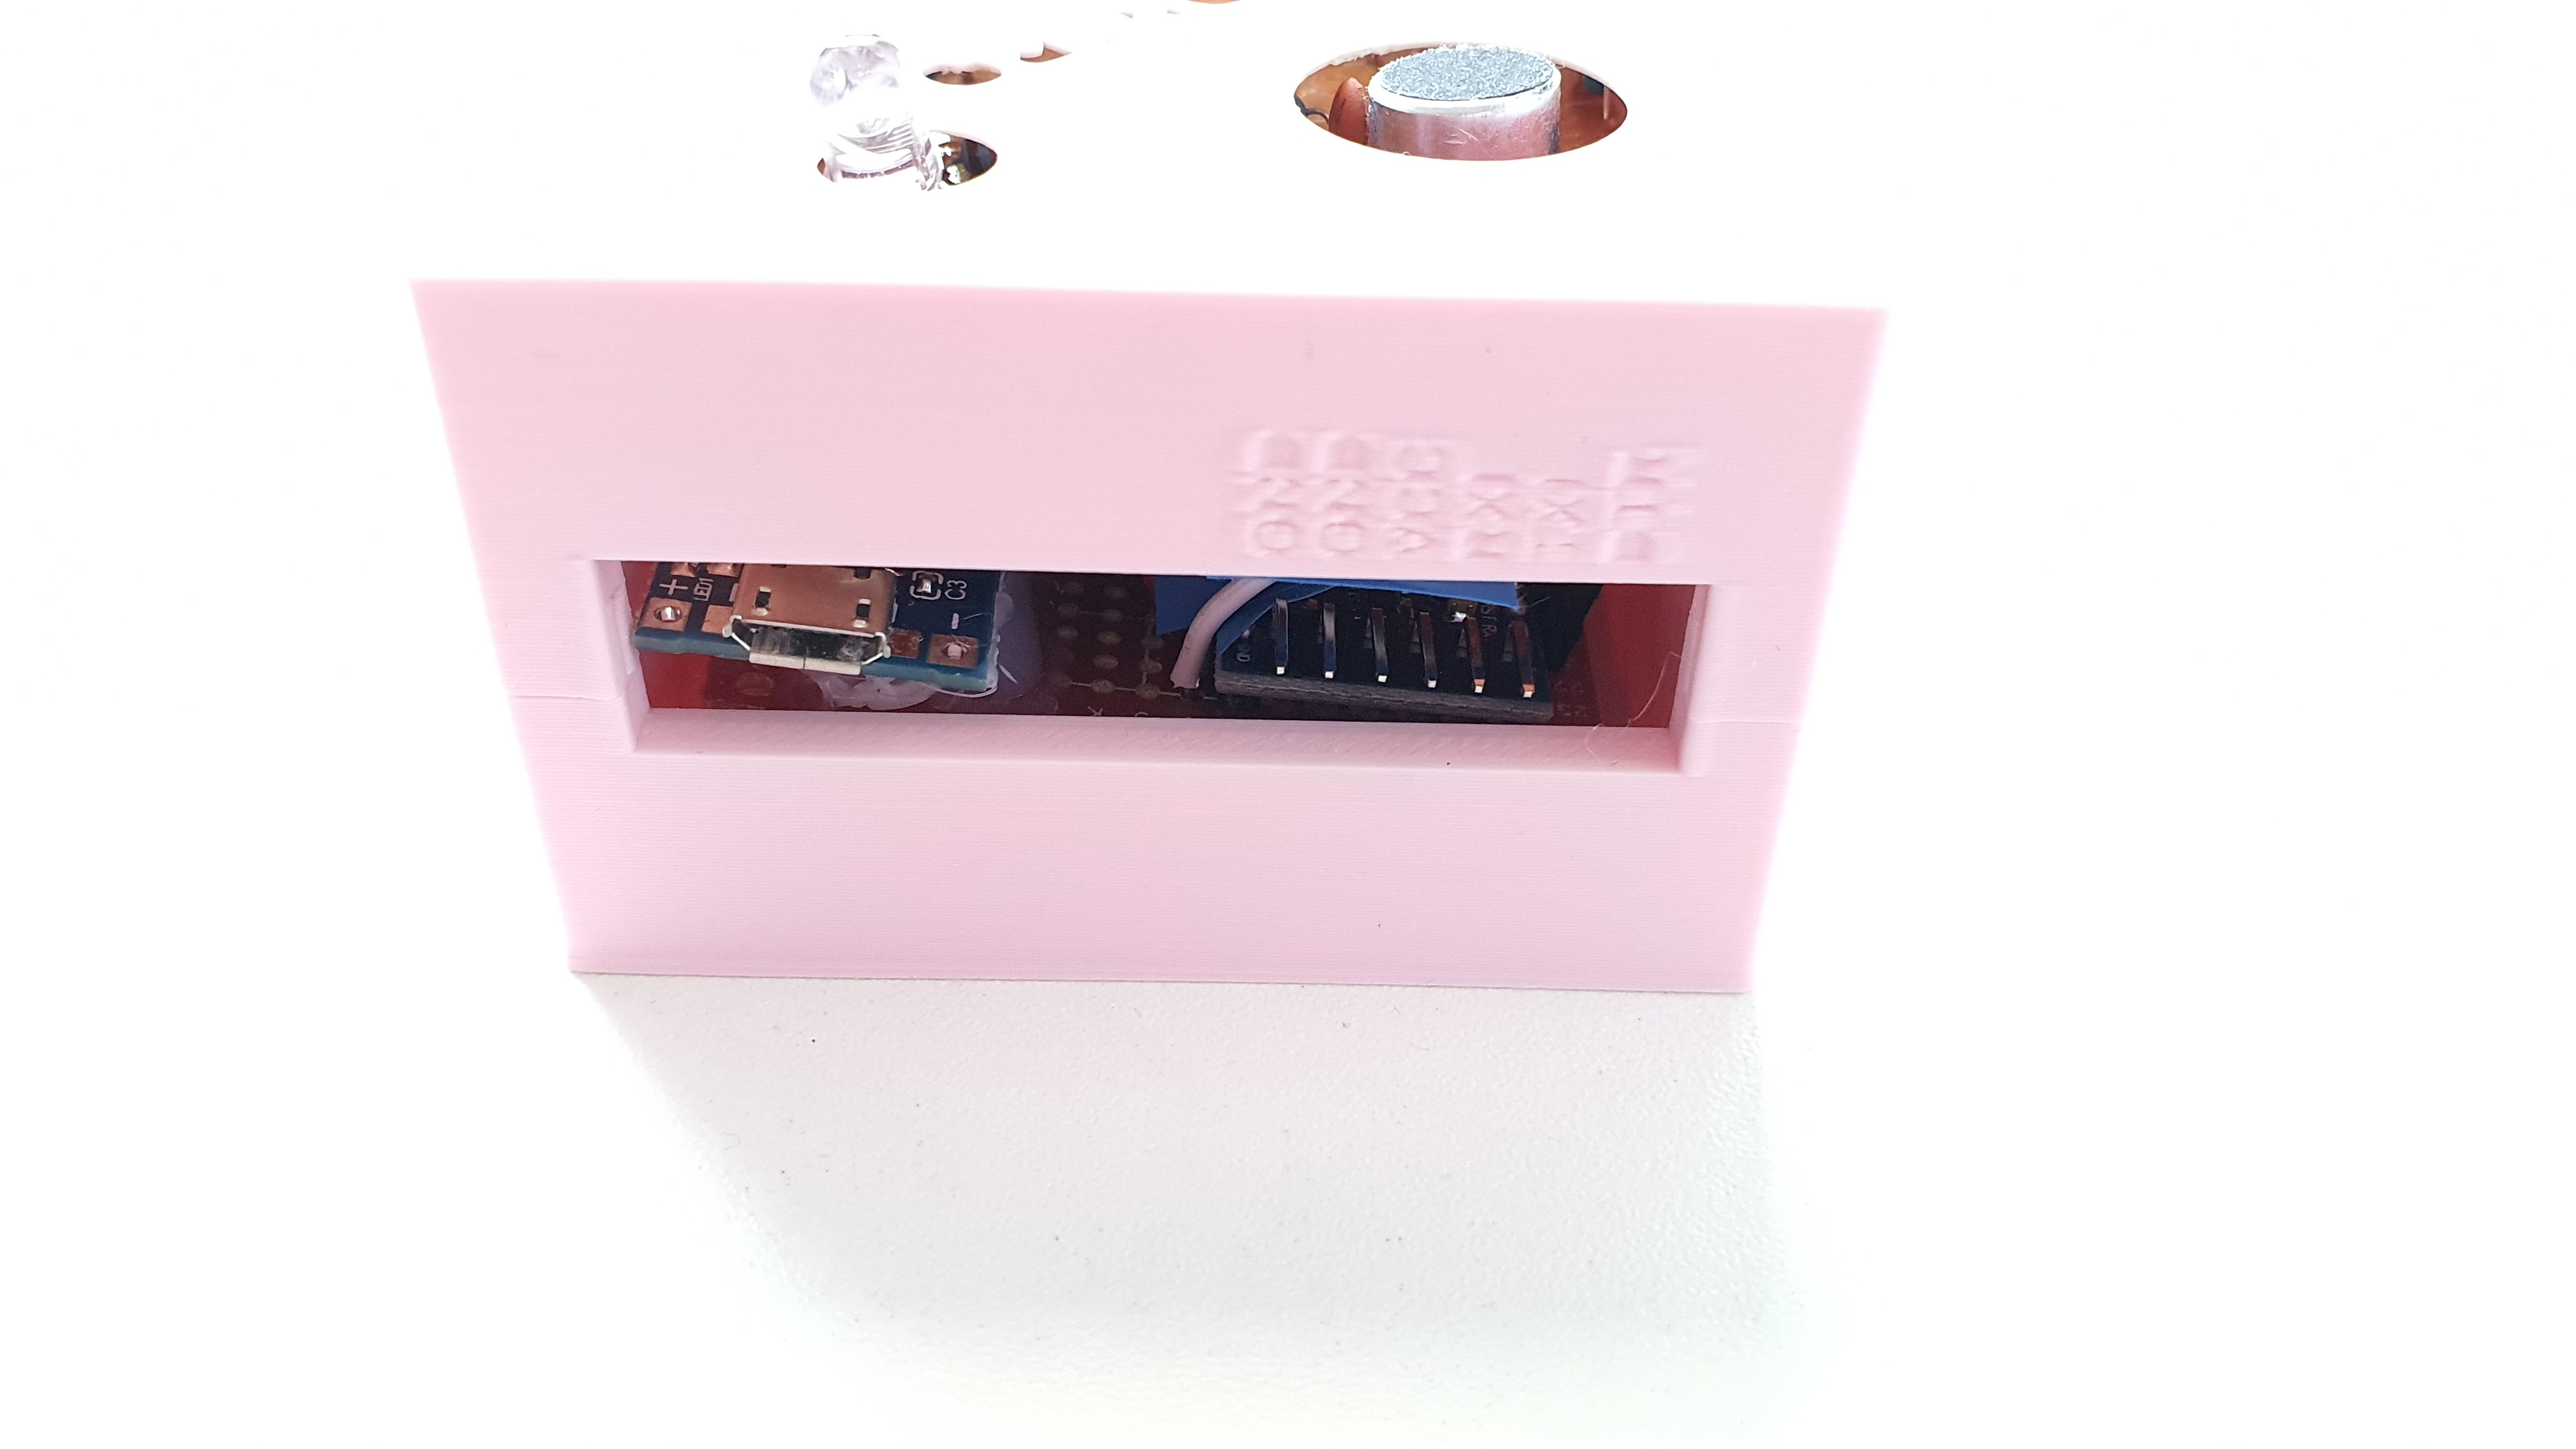
\includegraphics[width=\textwidth]{obr/obalkonektory.jpg}}
\caption{model ovládača zadná strana.}\label{OBRAZOK 1.6}
\end{figure}

\begin{figure}[!tbh]
\centering
\fbox{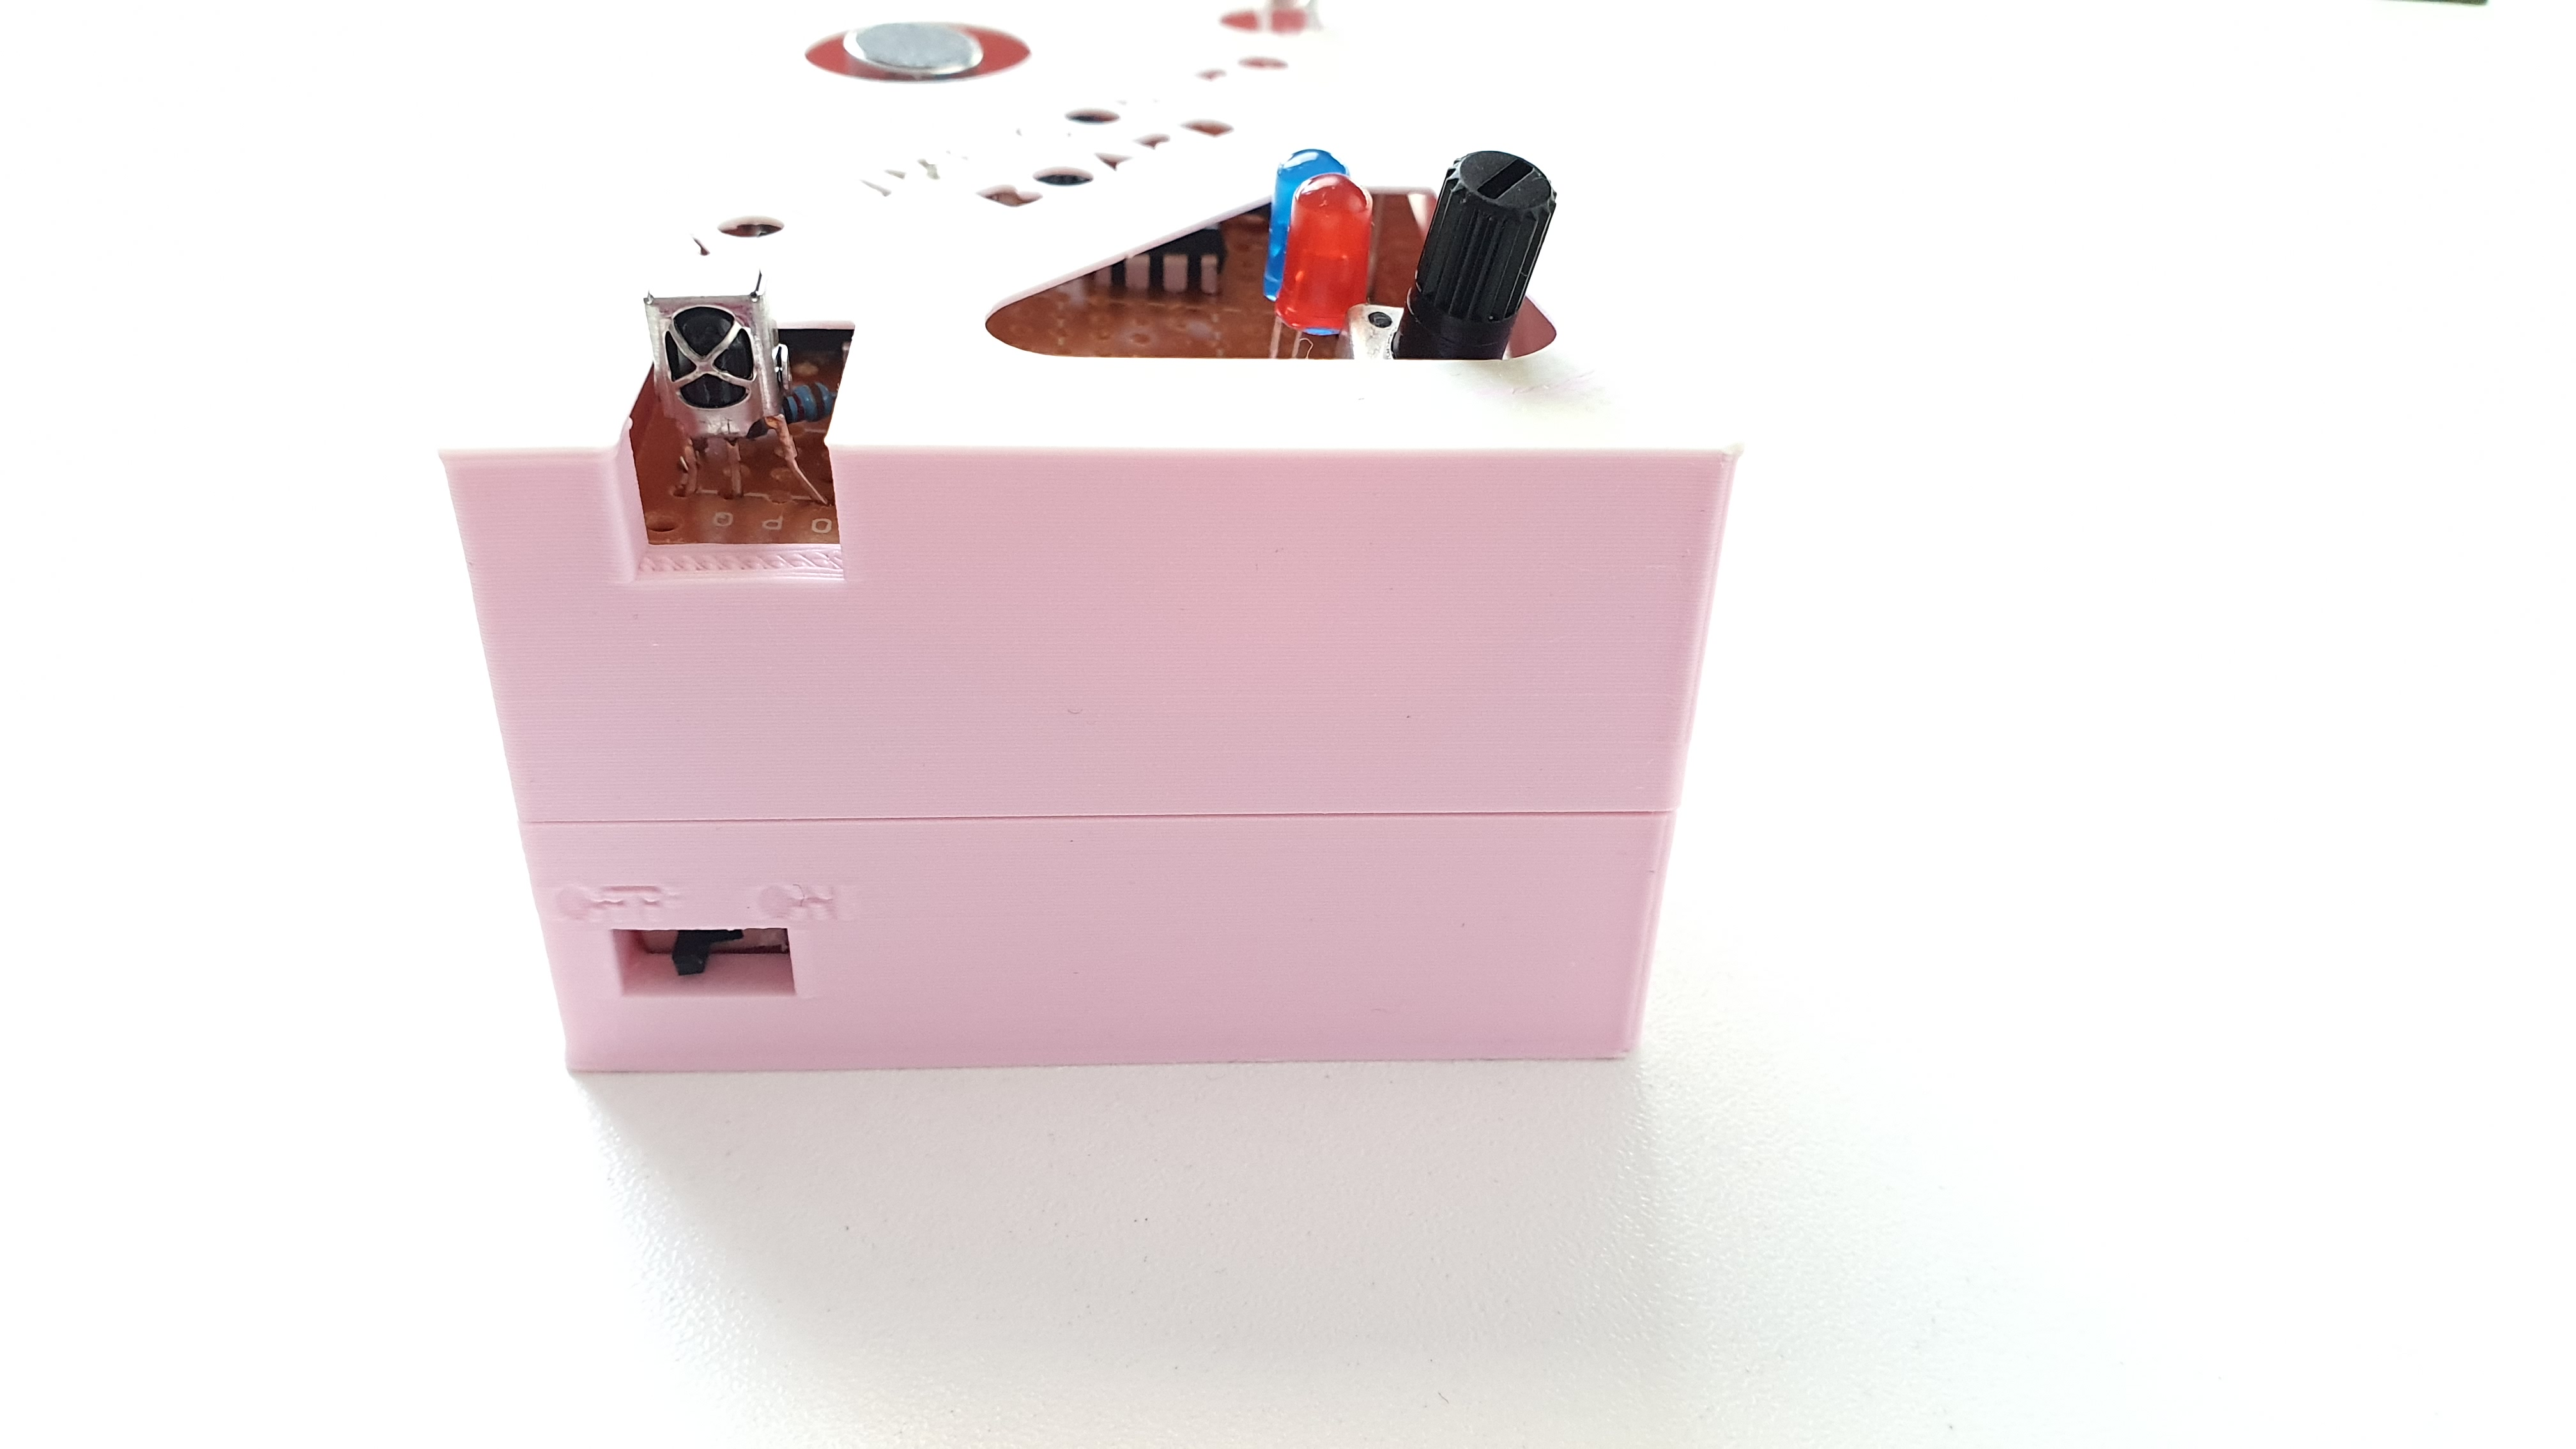
\includegraphics[width=\textwidth]{obr/obalkraj.jpg}}
\caption{model ovládača predná strana.}\label{OBRAZOK 1.7}
\end{figure}

Kvôli zabezpečeniu všetkých komponentov sme sa rozhodli vyrobiť pre náš ovládač hlasitosti aj obal ktorý bol vytlačený na 3D tlačiarni. Obal má na vrchnej strane výrezy pre všetky potrebné komponenty ako aj popisy funkcii akčných členov systému(potenciometrov). Z bočnej strany obalu je výrez pre vypínač s ktorým sa dá zariadenie vypnúť a zapnúť. Z druhej strany je výrez pre nabíjanie batérie a piny pre pripojenie Arduina ku počítaču.


\begin{figure}[!tbh]
\hfill
\subfigure[vrchná strana prototypovej dosky.]{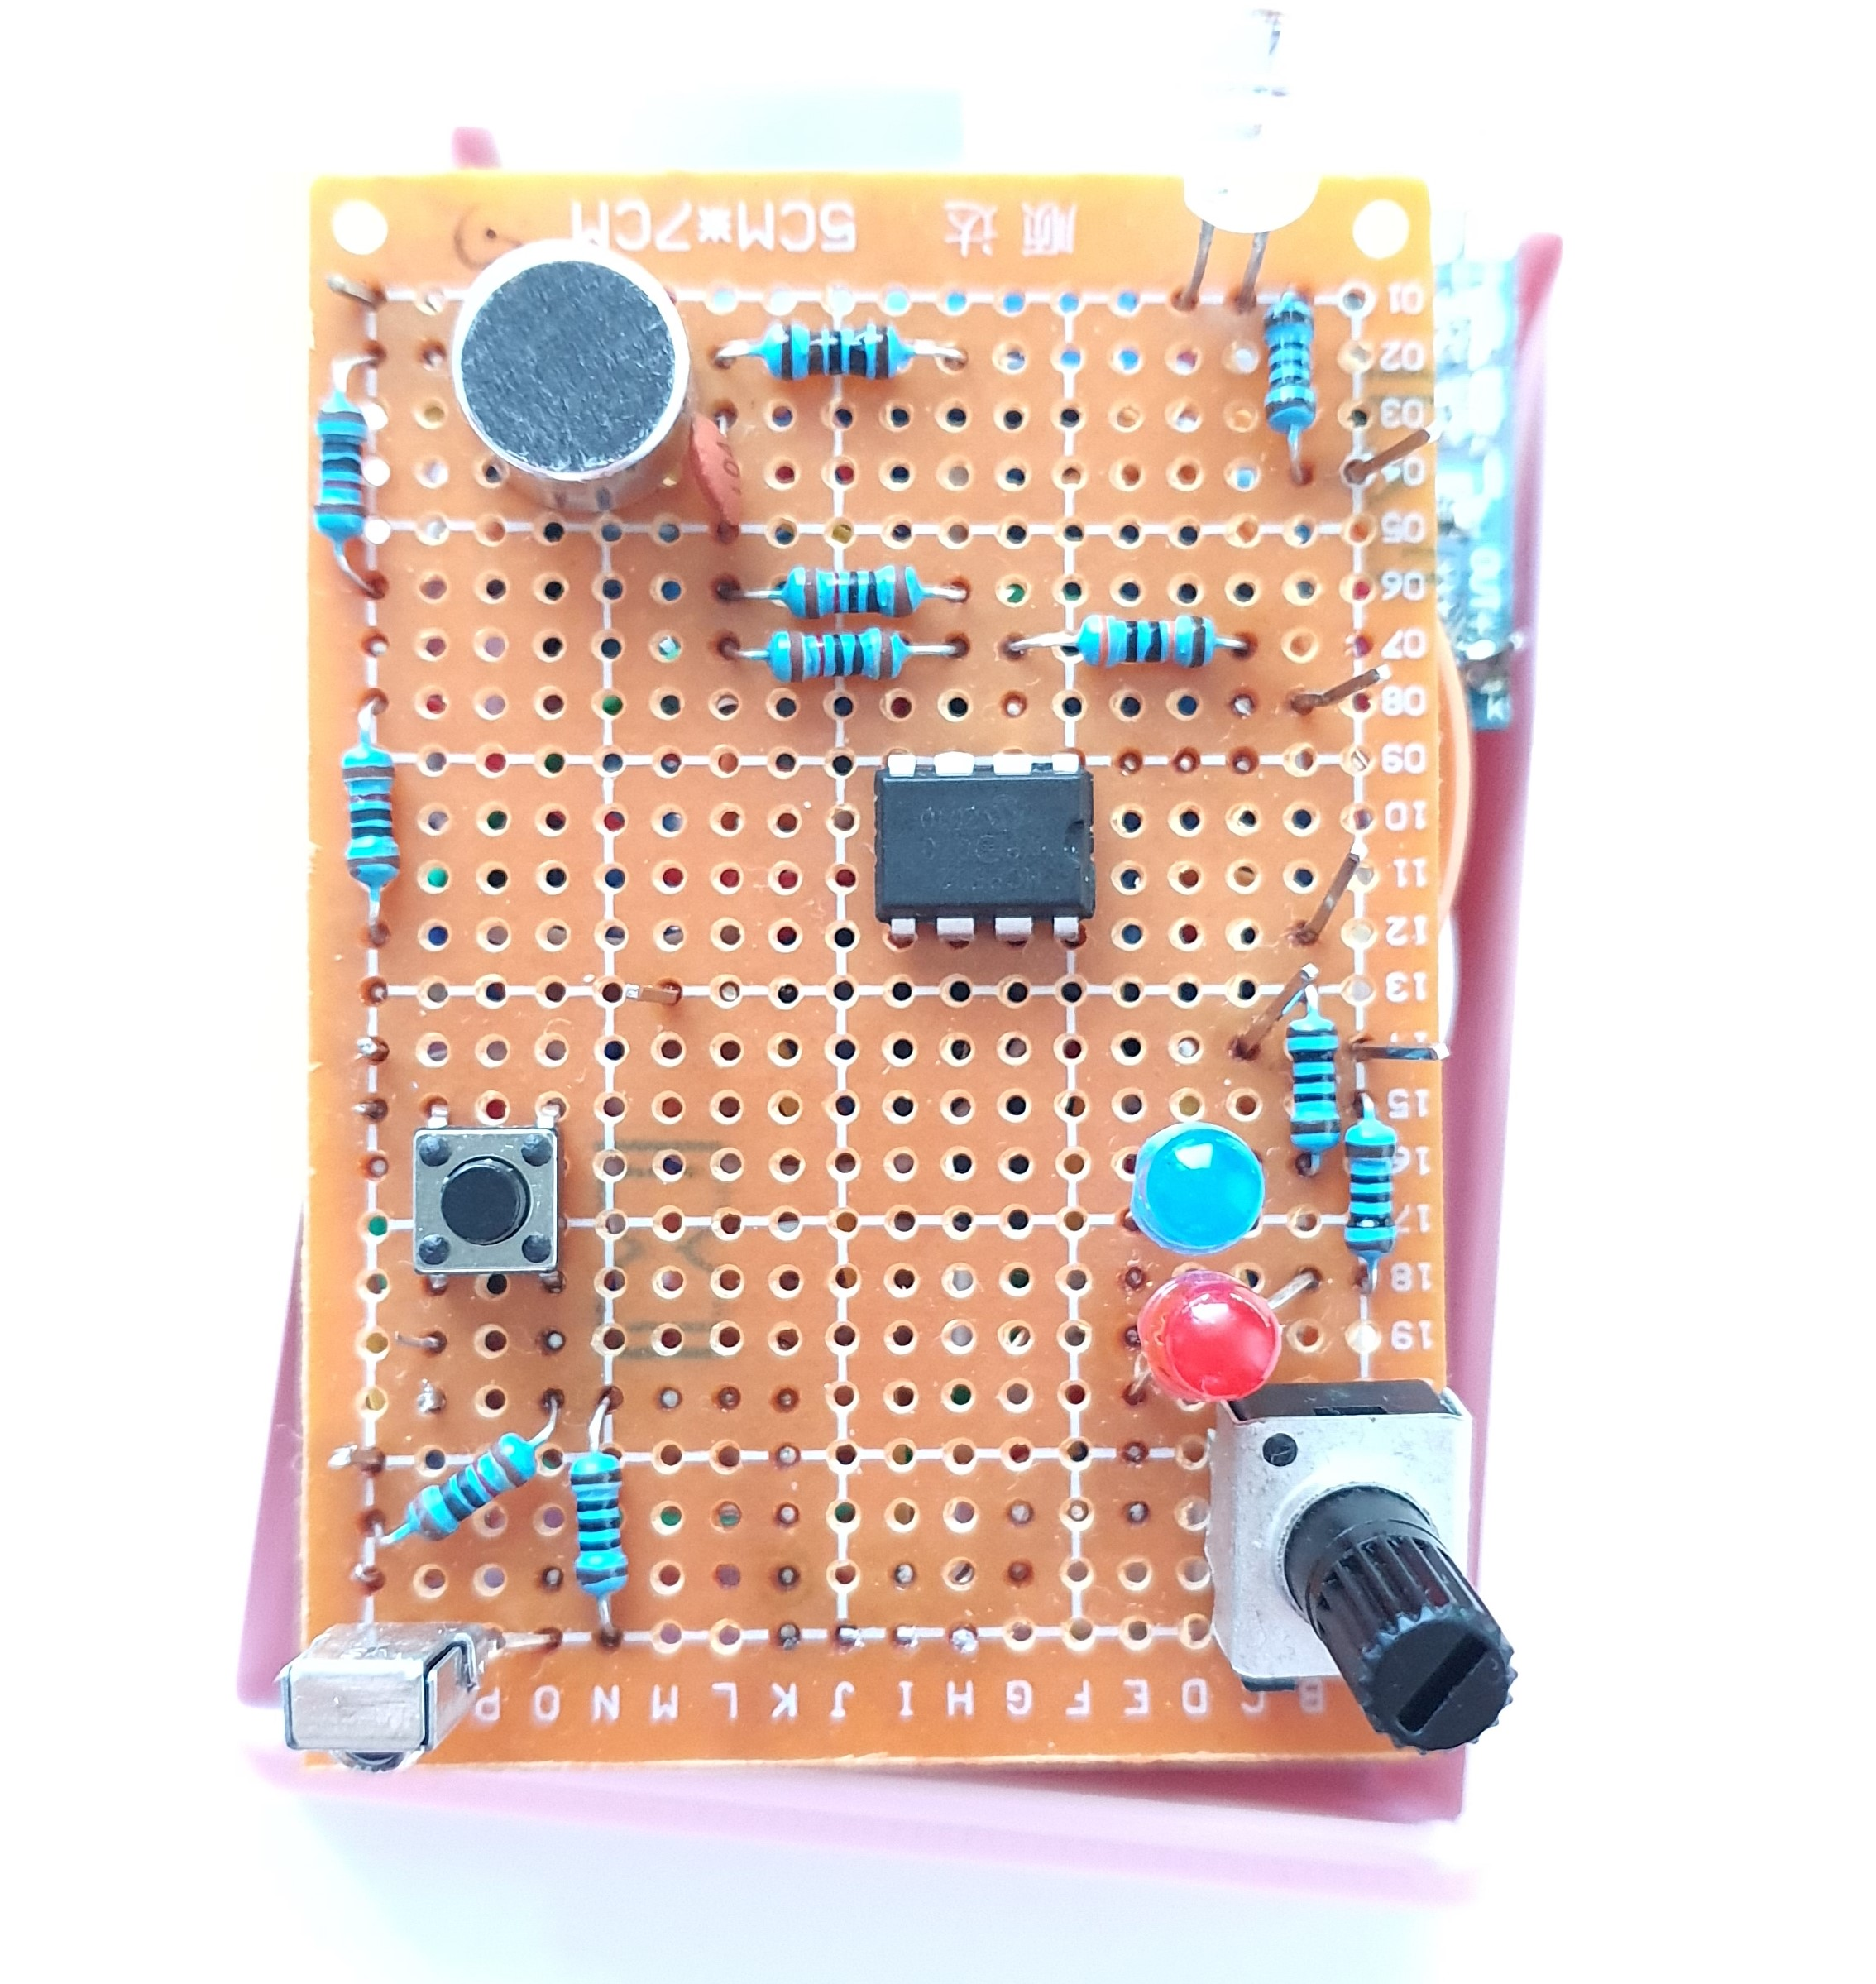
\includegraphics[width=7cm]{obr/pajkahore.jpg}}
\hfill
\subfigure[spodná strana spojov]{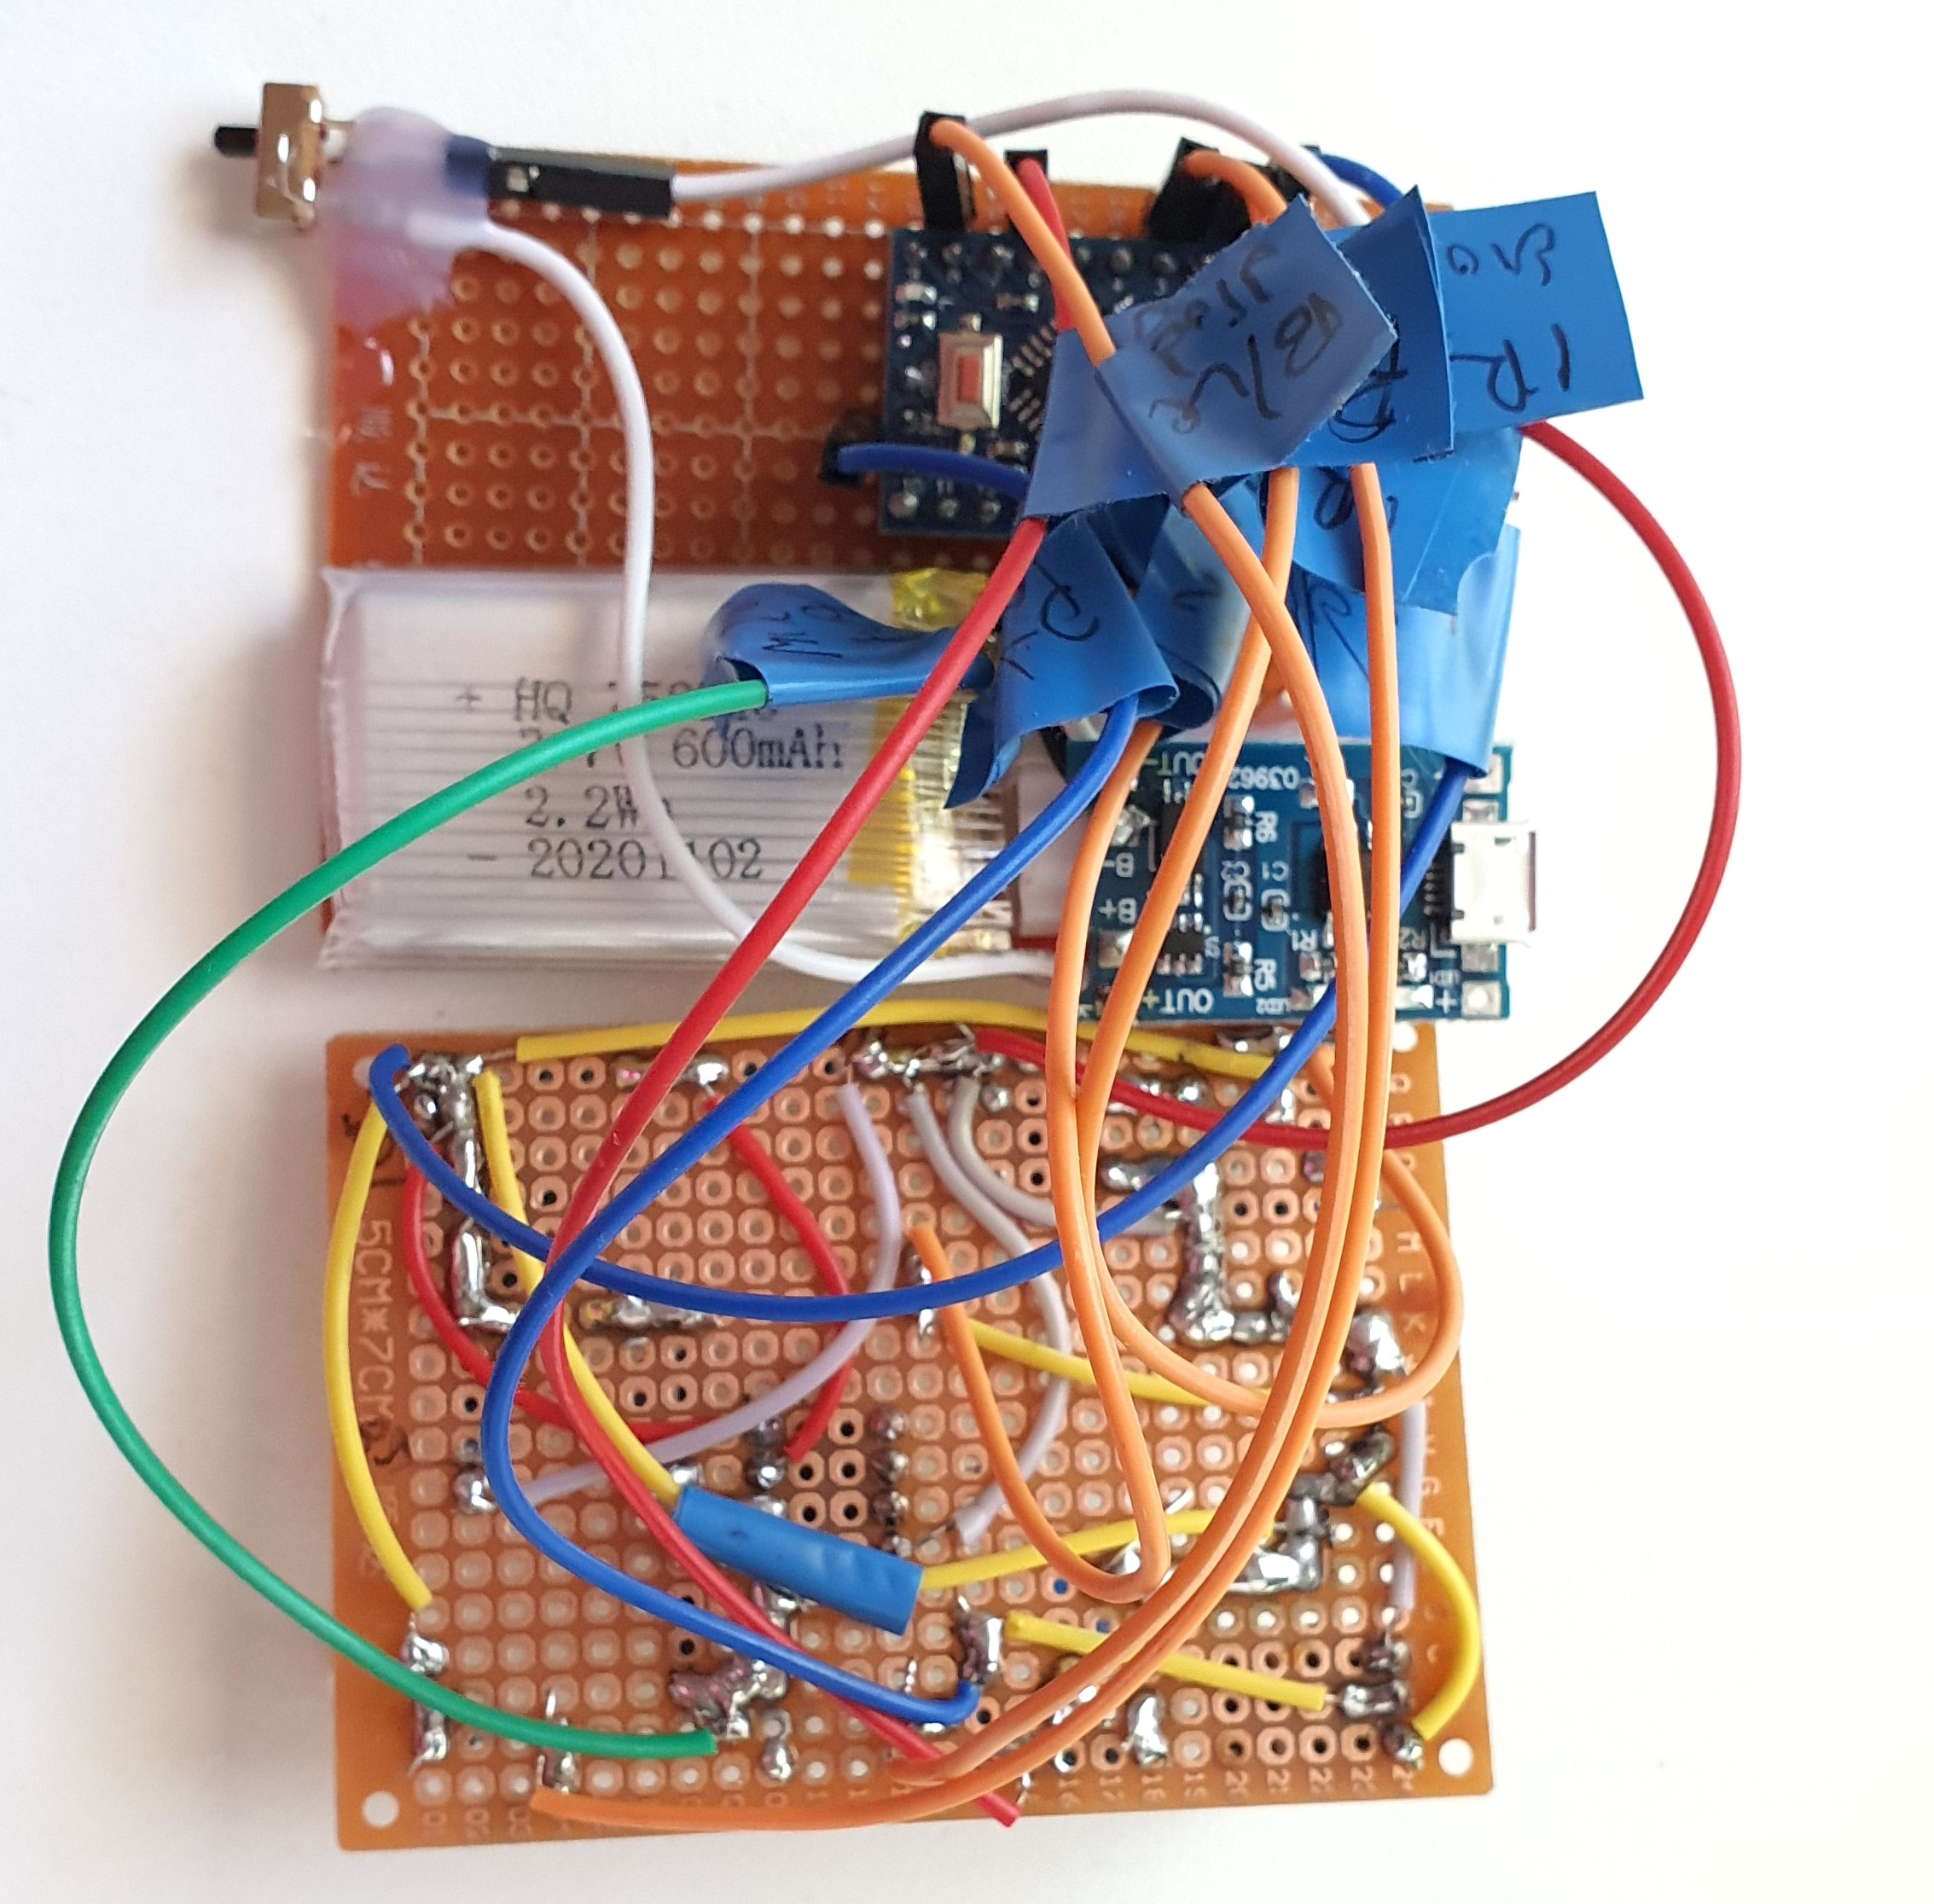
\includegraphics[width=7cm]{obr/pajkavsetko.jpg}}
\hfill
\caption{zapojenie pomocou jednostrannej prototypovej dosky}\label{OBRAZOK 1.8}
\end{figure}



\chapter{kód}
\section{Vysvetlenie kódu}

Pre správne fungovanie zariadenia sme potrebovali veľa funkcií na spracovanie signálu z mikrofónu do formy, s ktorou by sme mohli pracovať.

\section{Zero()}

Prvá funkcia potrebná na analýzu signálu je funkcia zero(). Jej úlohou je nájsť nulovú hladinu, číslo okolo ktorého oscilujú hodnoty signálu prijatého z mikrofónu. Princíp je nasledovný: do pomocnej premennej sum ukladá 5000 nameraných hodnôt takým spôsobom, že ich sčítava dohromady. Na konci tohto cyklu vydelí konečné číslo počtom nameraných hodnôt, čím získame priemer, ktorý sa zároveň rovná nulovej hladine. Táto funkcia sa vykoná v setupe(). 

\begin{lstlisting}

void zero() {
  float sum=0;
  int x;
  int i=0;
 while ( i < 5000) {
  x=analogRead(ReadPin);
  sum=sum+x;
  i++;
  }
  zerolevel=sum/5000.;
  }

\end{lstlisting}

\section{Maxvolume()}

Ďalšou dôležitou funkciou je funkcia maxvolume(). Jej úlohou je na konkrétnych intervaloch zisťovať maximálnu hodnotu signálu. Túto hodnotu si drží uloženú v premennej u po dĺžku hľadania novej hodnoty na ďalšom intervale rovnakej dĺžky. Táto funkcia je pre analýzu signálu veľmi dôležitá lebo pomocou nej môžeme signál upraviť do formy, v ktorej budeme vedieť overovať či hlasitosť už prekročila nami určenú hladinu hlasitosti. 

\begin{lstlisting}

void maxvolume(int mic) {
  currentMillis = millis();
  Umaxval=zerolevel;
  if (mic>Umaxval) {Umaxval=mic;}
  if (currentMillis - startMillis >= period1)
  {
     u=Umaxval;
    startMillis = currentMillis;
    Umaxval=zerolevel;
  }
}

\end{lstlisting}


\begin{figure}[!tbh]
\centering
\fbox{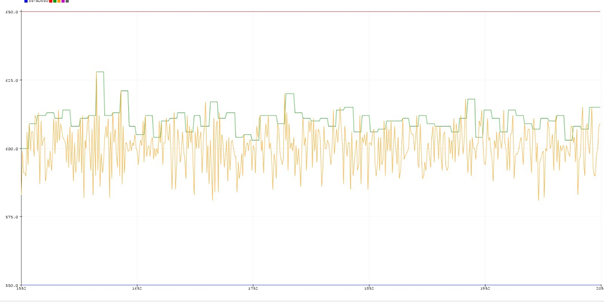
\includegraphics[width=\textwidth]{obr/graf1.png}}
\caption{Výstup mikrofónu pri intervale merania 20 ms.}\label{OBRAZOK 2.1}
\end{figure}

\begin{figure}[!tbh]
\centering
\fbox{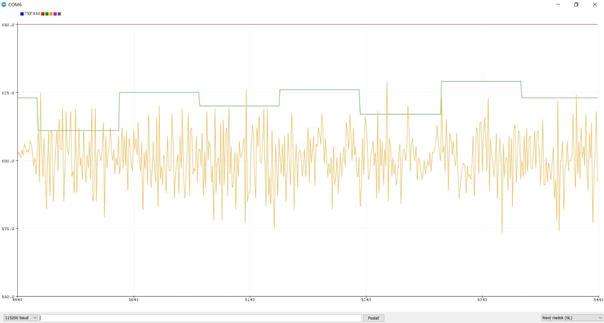
\includegraphics[width=\textwidth]{obr/graf2.png}}
\caption{Výstup mikrofónu pri intervale merania 100 ms.}\label{OBRAZOK 2.2}
\end{figure}


\section{Volume()}

Funkcia volume() slúži na zvyšovanie a znižovanie hlasitosti televízora. Kontroluje, či hodnota signálu (u) prekročila nami určenú maximálnu alebo minimálnu prípustnú hladinu. Ak táto situácia nastane počká určitý interval – period2 – a po jeho uplynutí znova overí podmienku. Toto slúži ako ochrana pred chybami, ktoré sa môžu vyskytnúť v priebehu signálu ale taktiež nám umožňuje nastavovať rýchlosť reakcie na zmenu hlasitosti. Ak podmienka platí aj po overení, zariadenie pomocou IR led pošle signál televízoru, ktorý hlasitosť buď zvýši alebo zníži.

 \begin{lstlisting}
void volume(int u){
 if (u < minval){
   currentmill = millis();
      if (currentmill - startmill >= period2)
         {
     digitalWrite(8, HIGH);
     IrSender.sendNEC(0x4,0x2,0);
     startmilll= millis();
   YieldDelay(100);
    digitalWrite(8, LOW);
  startmill = currentmill;
   }
  }
if (u > maxval ){
currentmill = millis();
if (currentmill - startmill >= period2)
     {
     digitalWrite(6, HIGH);
     IrSender.sendNEC(0x4,0x3,0);
    YieldDelay(100);
    digitalWrite(6, LOW);
     startmill = currentmill;
 }
}
}

\end{lstlisting}

Nasledujúce funkcie slúžia na ovládanie a nastavovanie parametrov programu pomocou potenciometrov.


\section{Volumelevel()}

Pomocou tejto funkcie si cez potenciometer dokážeme nastaviť aktuálnu výšku maximálnej (maxval) a minimálnej (minval) prípustnej hladiny hlasitosti bez toho by sme prepisovali program. V programe si musíme len nastaviť hodnoty, v ktorých sa budú môcť dané hodnoty pohybovať a maximálnu a minimálnu hodnotu získanú z potenciometra.

 \begin{lstlisting}
void volumelevel() {
  int MAXVAL_maxlevel = zerolevel + 60;
  int MAXVAL_minlevel = zerolevel + 10;
  int MINVAL_maxlevel = zerolevel + 30;
  int MINVAL_minlevel = zerolevel + 5;

  int minpot=0;
  int maxpot=660;
  float x=analogRead(LevelPin);

  maxval=((x/(maxpot-minpot))*(MAXVAL_maxlevel-MAXVAL_minlevel))+MAXVAL_minlevel;

  minval=((x/(maxpot-minpot))*(MINVAL_maxlevel-MINVAL_minlevel))+MINVAL_minlevel;
  }

\end{lstlisting}

\section{Reactiontime()}

Táto funkcia slúži na nastavovanie rýchlosti reakcie zariadenia na zmenu signálu z mikrofónu pomocou potenciometra v reálnom čase. Tak isto ako vo funkcii volumelevel() si v programe musíme nastaviť hodnoty, v ktorých intervale sa budeme pri nastavovaní pohybovať – maxperiod a minperiod. Tiež si nastavíme maximálnu a minimálnu hodnotu získanú z potenciometra.

  \begin{lstlisting}
void reactiontime () {
  int minpot=0;
  int maxpot=660;
  float x=analogRead(Period2Pin);

  int maxperiod = 5000;
  int minperiod = 500;

  period2 = ((x/(maxpot-minpot))*(maxperiod-minperiod))+minperiod;
  }

\end{lstlisting}

V loope programu teda len voláme dané funkcie až na zero() , ktorá je v setupe.
%


V časti texty, na podstránke indexx.php, nájde užívateľ nadpis a dátum publikácie článkov obr.\ref{OBRAZOK 1.2}. Po kliknutí na nadpis, sa užívateľovi zobrazí len požadovaný článok, ktorý sa rozvinie a zobrazí v celej dĺžke obr.\ref{OBRAZOK 1.3}. Textová/blogová časť kódu a jeho fungovanie bolo inšpirované open-source\footnote[2]{Open-source je zo všeobecného pohľadu akákoľvek informácia, ktorá je dostupná verejnosti bez poplatku(s voľným prístupom), s ohľadom na fakt, že jej voľné šírenie zostane zachované.} projektom\cite{blog}.

\begin{figure}[!tbh]
\centering
\setlength{\fboxsep}{0pt}%
\setlength{\fboxrule}{1pt}%
\fbox{\includegraphics[width=\textwidth]{obr/texty_bez_text.png}}
\caption{Texty publikované na podstránke indexx.php.}\label{OBRAZOK 1.2}
\end{figure}

\begin{figure}[!tbh]
\centering
\setlength{\fboxsep}{0pt}%
\setlength{\fboxrule}{1pt}%
\fbox{\includegraphics[width=\textwidth]{obr/texty_s_text.png}}
\caption{Zobrazenie konkrétneho textu na podstránke indexx.php.}\label{OBRAZOK 1.3}
\end{figure}

\vspace{5cm}

V časti, foto, nájde užívateľ výber fotiek, ktoré sa klient rozhodol zdieľať obr.\ref{OBRAZOK 1.4}. Fotky sú uložené v radoch, po troch fotkách, a pri prejdení kurzorom nad fotku, sa užívateľovi zobrazí popis fotky obr.\ref{OBRAZOK 1.5}. Pri následnom kliknutí na fotku, sa konkrétna fotka maximalizuje(sú ale určené max. hodnoty šírky) a zobrazí sa aj príslušný nadpis a popis fotky obr.\ref{OBRAZOK 1.6}. Zobrazenie galérie, ako aj fotky v okne, je vykonávané pomocou java script kódu, využitého z open-source projektu\cite{Gallery}.

\begin{figure}[!tbh]
\centering
\setlength{\fboxsep}{0pt}%
\setlength{\fboxrule}{1pt}%
\fbox{\includegraphics[width=\textwidth]{obr/galeria.png}}
\caption{Fotky publikované na podstránke foto.php.}\label{OBRAZOK 1.4}
\end{figure}

\begin{figure}[!tbh]
\centering
\setlength{\fboxsep}{0pt}%
\setlength{\fboxrule}{1pt}%
\fbox{\includegraphics[width=\textwidth]{obr/galeria_nahlad.png}}
\caption{Náhľad popisu fotky na podstránke foto.php.}\label{OBRAZOK 1.5}
\end{figure}

\vspace{2cm}

V časti portfolko, na podstránke portfolio.php, nájde užívateľ jednoduché okno, v ktorom sa zobrazuje PDF súbor portfólia klienta obr.\ref{OBRAZOK 1.7}. Užívateľ si môže PDF súbor prezerať, alebo stiahnuť priamo zo stránky.

\begin{figure}[!tbh]
\centering
\setlength{\fboxsep}{0pt}%
\setlength{\fboxrule}{1pt}%
\fbox{\includegraphics[width=\textwidth]{obr/galeria_zobrazenie.png}}
\caption{Zobrazenie konkrétnej fotky na podstránke foto.php.}\label{OBRAZOK 1.6}
\end{figure}



\begin{figure}[!tbh]
\centering
\setlength{\fboxsep}{0pt}%
\setlength{\fboxrule}{1pt}%
\fbox{\includegraphics[width=\textwidth]{obr/portfolko.png}}
\caption{Portfólio na podstránke portfolio.php.}\label{OBRAZOK 1.7}
\end{figure}






%\include{Funkcie stránky}
%\include{Fungovanie stránky}
\chapter{Záver}

Cieľom projektu bolo navrhnúť a skonštruovať zariadenie na úpravu hlasitosti televízora, ktorý sme splnili, až na technický problém pri finálnom testovaní.

Pri postupe sme najprv navrhli po častiach jednotlivé funkcie kódu ktoré sme testovali na breadboarde. Jediná funkcia ktorá sa nám nepodarila realizovať bola predošle spomenutá funkcia na ukladanie kódov zmeny hlasitosti. Táto funkcia by iba vylepšila zariadenie a nebola kľúčová pre fungovanie, preto sme sa rozhodli ju vynechať. Keď sme mali pripravené všetky časti kódu, spojili sme ich do jedného programu a otestovali sme ho na prvom prototype – zapojenie na breadboarde. Po ďalších úpravách sme zostavili prototyp 2 aj s obalom vyrobeným v 3D tlačiarni.

Hlavný problém, s ktorým sme sa stretli pri tomto projekte bola obmedzená komunikácia a lockdown, kvôli ktorému bol znemožnený osobný kontakt a online komunikácia bola nedostačujúca.

Aj napriek týmto komplikáciám sme si overili schopnosť využitia získaných vedomostí počas tohto semestra, čo považujeme za významný osobný prínos.





%%%%%%% Koniec %%%%%%%%
\bibliographystyle{plain}
\addcontentsline{toc}{chapter}{Literat\'{u}ra}
\bibliography{bibliog}
\end{document}
